%%%%%%%%%%%%%%%%%%%%%%%%%%%%%%%%%%%%%%%%%%%%%%%%%%%
%% LaTeX book template                           %%
%% Author:  Amber Jain (http://amberj.devio.us/) %%
%% License: ISC license                          %%
%%%%%%%%%%%%%%%%%%%%%%%%%%%%%%%%%%%%%%%%%%%%%%%%%%%

\documentclass[a5paper,11pt]{book}
\usepackage[T1]{fontenc}
\usepackage[utf8]{inputenc}
\usepackage{lmodern}
\usepackage{pifont,kantlipsum}
\usepackage{subfig}
\usepackage{float}
\newcommand*{\altasterism}{\vspace*{1em plus .5em minus .5em}\noindent\hspace*{\fill}\ding{104}\hspace*{\fill}}
%%%%%%%%%%%%%%%%%%%%%%%%%%%%%%%%%%%%%%%%%%%%%%%%%%%%%%%%%
% Source: http://en.wikibooks.org/wiki/LaTeX/Hyperlinks %
%%%%%%%%%%%%%%%%%%%%%%%%%%%%%%%%%%%%%%%%%%%%%%%%%%%%%%%%%
\usepackage{hyperref}
\usepackage{graphicx}
\usepackage[english, norsk]{babel}
\usepackage{verse}


%%%%%%%%%%%%%%%%%%%%%%%%%%%%%%%%%%%%%%%%%%%%%%%%%%%%%%%%%%%%%%%%%%%%%%%%%%%%%%%%
% 'dedication' environment: To add a dedication paragraph at the start of book %
% Source: http://www.tug.org/pipermail/texhax/2010-June/015184.html            %
%%%%%%%%%%%%%%%%%%%%%%%%%%%%%%%%%%%%%%%%%%%%%%%%%%%%%%%%%%%%%%%%%%%%%%%%%%%%%%%%
\newenvironment{dedication}
{
   \cleardoublepage
   \thispagestyle{empty}
   \vspace*{\stretch{1}}
   \hfill
   \begin{minipage}[t]{0.66\textwidth}
   \raggedright
}
{
   \end{minipage}
   \vspace*{\stretch{3}}
   \clearpage
}

%%%%%%%%%%%%%%%%%%%%%%%%%%%%%%%%%%%%%%%%%%%%%%%%
% Chapter quote at the start of chapter        %
% Source: http://tex.stackexchange.com/a/53380 %
%%%%%%%%%%%%%%%%%%%%%%%%%%%%%%%%%%%%%%%%%%%%%%%%
\makeatletter
\renewcommand{\@chapapp}{}% Not necessary...
\newenvironment{chapquote}[2][2em]
  {\setlength{\@tempdima}{#1}%
   \def\chapquote@author{#2}%
   \parshape 1 \@tempdima \dimexpr\textwidth-2\@tempdima\relax%
   \itshape}
  {\par\normalfont\hfill--\ \chapquote@author\hspace*{\@tempdima}\par\bigskip}
\makeatother

%%%%%%%%%%%%%%%%%%%%%%%%%%%%%%%%%%%%%%%%%%%%%%%%%%%
% First page of book which contains 'stuff' like: %
%  - Book title, subtitle                         %
%  - Book author name                             %
%%%%%%%%%%%%%%%%%%%%%%%%%%%%%%%%%%%%%%%%%%%%%%%%%%%

% Book's title and subtitle
\title{\Huge \textbf{Lisbeths bok}}
% Author
\author{Tekst: Ane, Tor Håkon, Oline og Helene\\ Illustrasjoner: Helene og Oline}
%{\textsc{Ane, Jon, Tor Håkon, Helene, Ulrik og Agnes}}


\begin{document}

\frontmatter
\maketitle

%%%%%%%%%%%%%%%%%%%%%%%%%%%%%%%%%%%%%%%%%%%%%%%%%%%%%%%%%%%%%%%
% Add a dedication paragraph to dedicate your book to someone %
%%%%%%%%%%%%%%%%%%%%%%%%%%%%%%%%%%%%%%%%%%%%%%%%%%%%%%%%%%%%%%%
\begin{dedication}
Til mamma, mormor, og farmor Lisbeth
\end{dedication}

%%%%%%%%%%%%%%%%%%%%%%%%%%%%%%%%%%%%%%%%%%%%%%%%%%%%%%%%%%%%%%%%%%%%%%%%
% Auto-generated table of contents, list of figures and list of tables %
%%%%%%%%%%%%%%%%%%%%%%%%%%%%%%%%%%%%%%%%%%%%%%%%%%%%%%%%%%%%%%%%%%%%%%%%
\tableofcontents
\mainmatter


%%%%%%%%%%%
% Preface %
%%%%%%%%%%%
\chapter*{Forord}
\renewcommand{\baselinestretch}{1.5} 
I anledning at du har fylt 70 år har vi laget denne boken. Det er en samling med historier og bilder om deg, noen fra fantasien og andre fra virkeligheten.\\
Vi håper du setter pris på den og ønsker deg en fabelaktig feiring!\\


\begin{flushright}
\textit{Klemmer fra\\
Ane, Jon, Tor Håkon, Helene, Ulrik og Agnes}
\end{flushright}
\newpage
%%%%%%%%%%%%%%%%%%%%%%%%%%%%%%%%%%%%
% Give credit where credit is due. %
% Say thanks!                      %
%%%%%%%%%%%%%%%%%%%%%%%%%%%%%%%%%%%%
 
\section*{Takk}
Takk til Tor Håkon og Oline for timer med skriving av historier! Det har vært veldig gøy å være med på, og å få oppleve fantasien og skrivegleden dere har. Takk til Helene og Oline for flotte illustrasjoner. Takk til Odd for hjelp til å finne fram Lisbeths musikalske karriere.

%%%%%%%%%%%%%%%%
% NEW CHAPTER! %
%%%%%%%%%%%%%%%%
\chapter{Lisbeth fra Dalsnes}

\begin{chapquote}{Herbjørg Wassmo}
``Noen ganger koster det mer å være feig enn å hoppe uti og se hva som skjer.''
\end{chapquote}

\section{Dalsnes}
%Noe om Dalsnes, Mors gård. Bilder og kart?
\section{Søsknene Fredriksen}
%Bilder av alle søsknene


\chapter{Eventyrene til romfarer Dalsnes}
%\section{}
Det var en gang en veldig snill mormor som heter Lisbeth. Hun hadde oppdaget en helt ny planet.\\ Hun skulle egentlig på Pluto, men hun fikk noen problemer med motoren i romskipet. Så hun styrtet, men hun var magisk så hun overlevde.\\ Hun så seg rundt og oppdaget at alt var av godteri.\\
\begin{figure}[H]
    \centering
    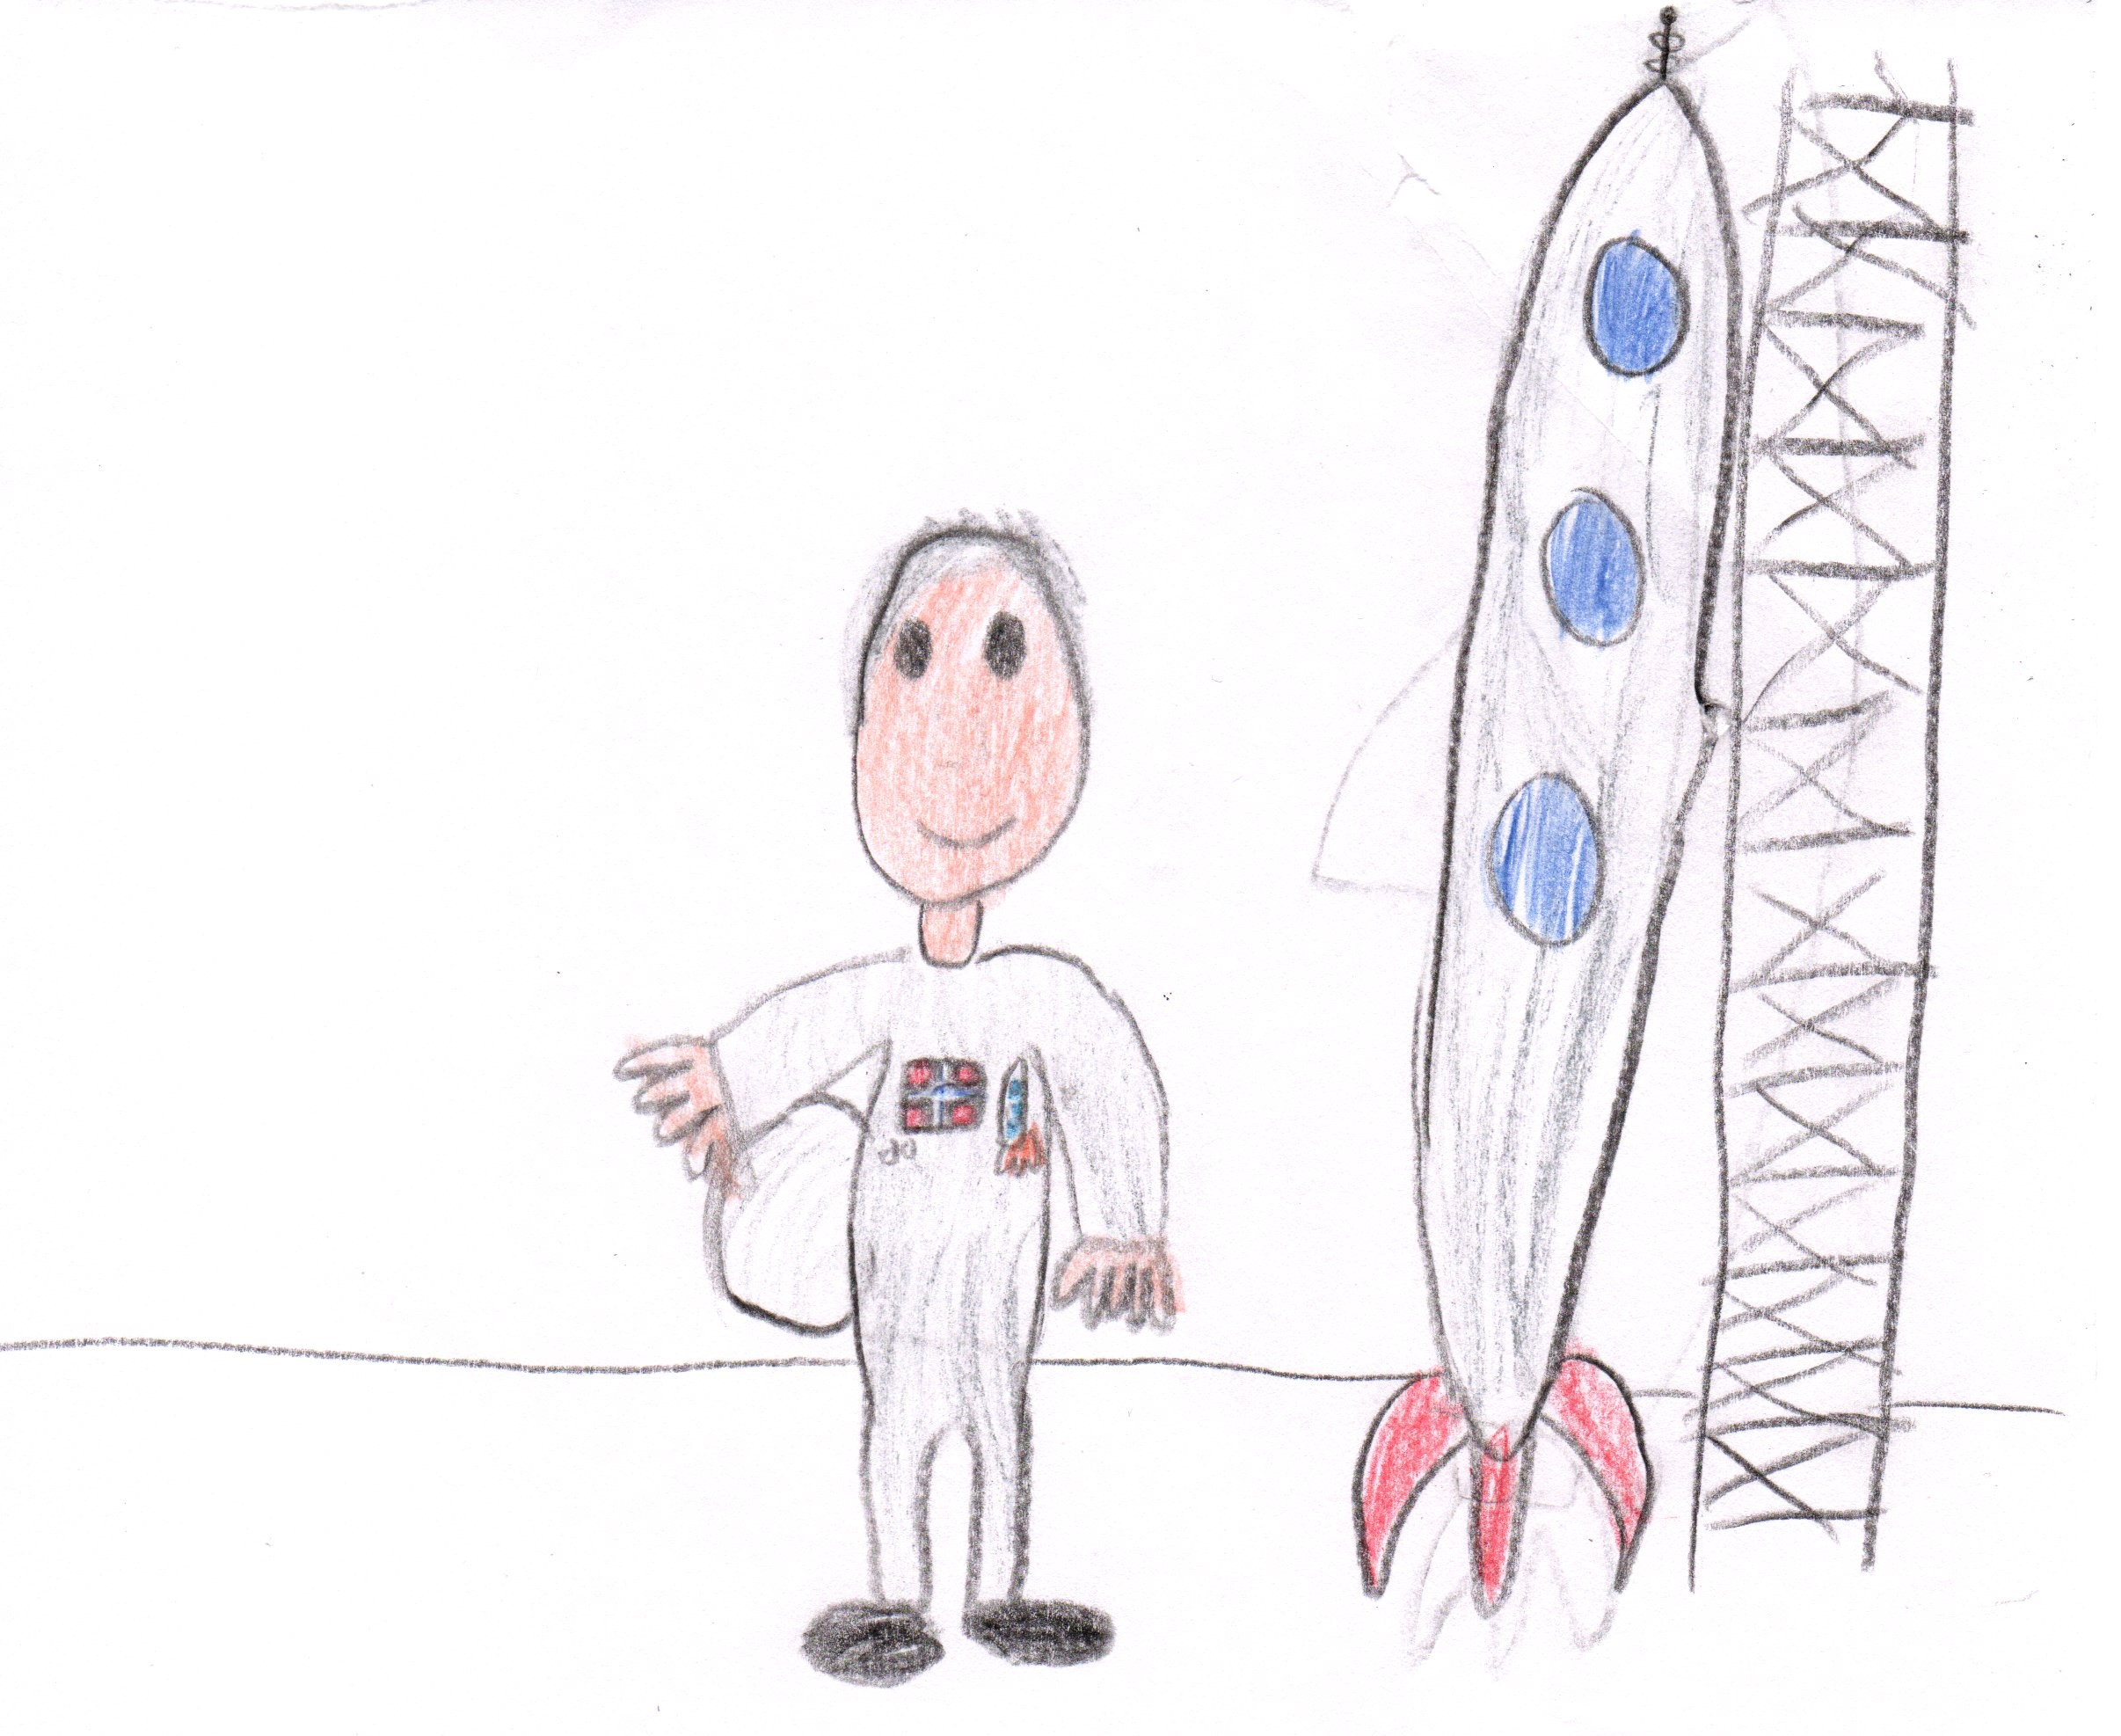
\includegraphics[width=0.8\textwidth]{illustrasjoner/Lisbethromfarer.jpg}
   \label{romfarer}
   \caption{Romfarer Dalsnes av Oline}
\end{figure}

Hun måtte finne på et navn til planeten. Hun fant på et morsomt navn. \textit{Knask og godt} var navnet  til planeten.\hfill \newline\\ 
Skyene var av sukkerspinn. Noen sukkerspinnskyer var rosa, noen var grønne og noen var blåe og de hadde strøssel. Stammen til trærene var av lakris og bladene var av sjokolade med grønn konditorfarge! Og den vakreste fossen av smeltet melkesjokolade rant rett ved siden av den ødelagte romskipet. Steinene var av marshmallow og husene var av pepperkaker.\\
\hfill \newline
Hun prøvde og ringe til folket i byen hennes, men det var ikke dekning på planeten. Så hun måtte bli der. Menneskene var ikke menesker, men seigmenn og de hadde ikke hunder og katter til kjæledyr men de hadde gummibjørner som kjæledyr.\\
\hfill \newline 
Hun lagde seg et hus av pepperkake og flyttet inn i byen. Hun fikk noen venner i byen fordi selv om  det bare var seigmenner i byen kunne de snakke.\\
\hfill \newline
Hun var så snill at hun fikk snill-superkrefter! Det kom ofte meteoritter til byen men hun stoppet dem med snill-superkreftene sine. Hun kunne fly og hun ville oppdage flere matrealer fra andre planeter, men hun lovte og komme tilbake. \\
\hfill \newline
Hun oppdaget en planet av myke ting hun kalte den Kose-planeten og der var det allemulige ting som var helt myke. Og hun oppdaget en planet som hun kalte Ferie-planeten, der var det bare skole på torsdager. Der holt barna på med og lage fine ting i stede for og ha skole. Etter det dro hun til en ny planet hun kalte den Regnbue-planeten. Der var det kjempe mange regnbuer og de fleste var veldig store!
%%%%%%%%%%%%%%%%%%%%%%%%%%%%%%%%%%%%%%%%%%%%%%%%%%%%%%%
\section{Monsterplaneten}
\begin{figure}[H]
    \centering
    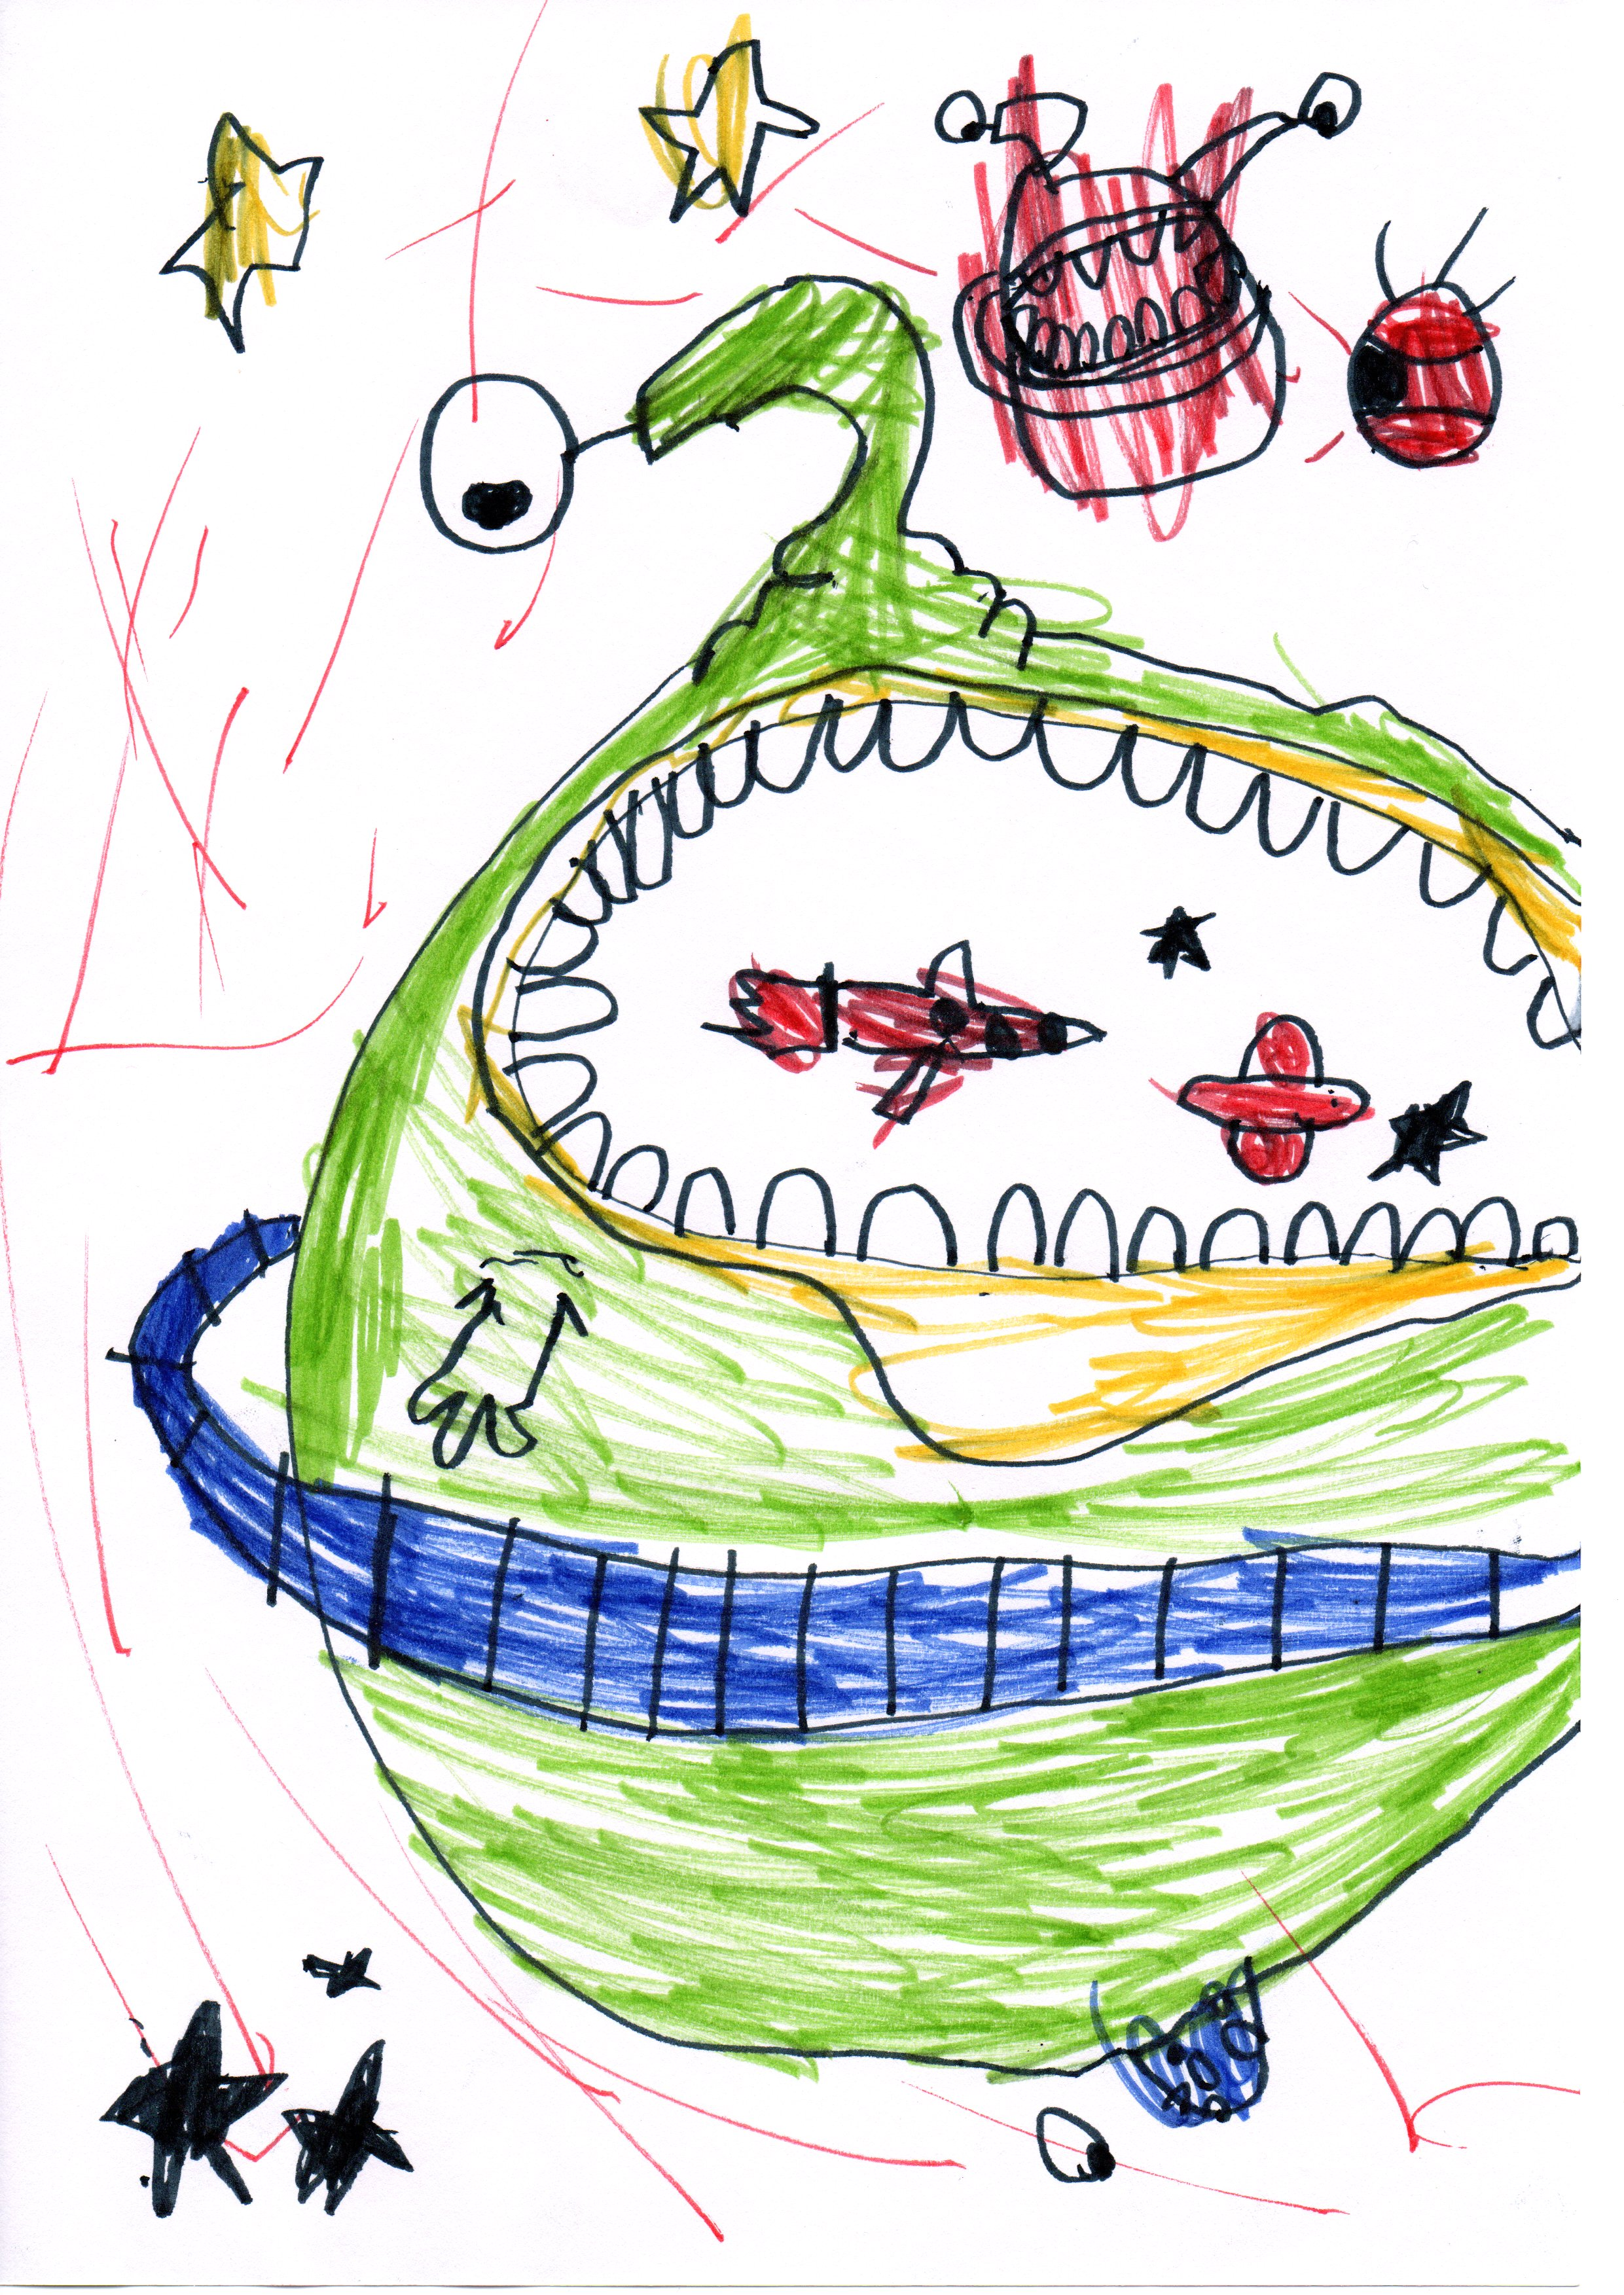
\includegraphics[scale=0.30]{illustrasjoner/Universmonster.jpg}
   \label{Planetmonster}
   \caption{Planetmonster av Helene}
\end{figure}
Hun dro til en stor monsterplanet full av monster.\\
\hfill \\
Planeten var et monster også.\\
\hfill \\
På monster-planeten var det et monster som het Kalle Monsteret.\\
\hfill \\
Kalle monsteret var dronningen til innbyggerne som kaltes Mipmiper.\\ \hfill \\
Kalle monsteret kan kalle på Mipmiperne.\\ \hfill \\

\begin{figure}[H]
    \centering
    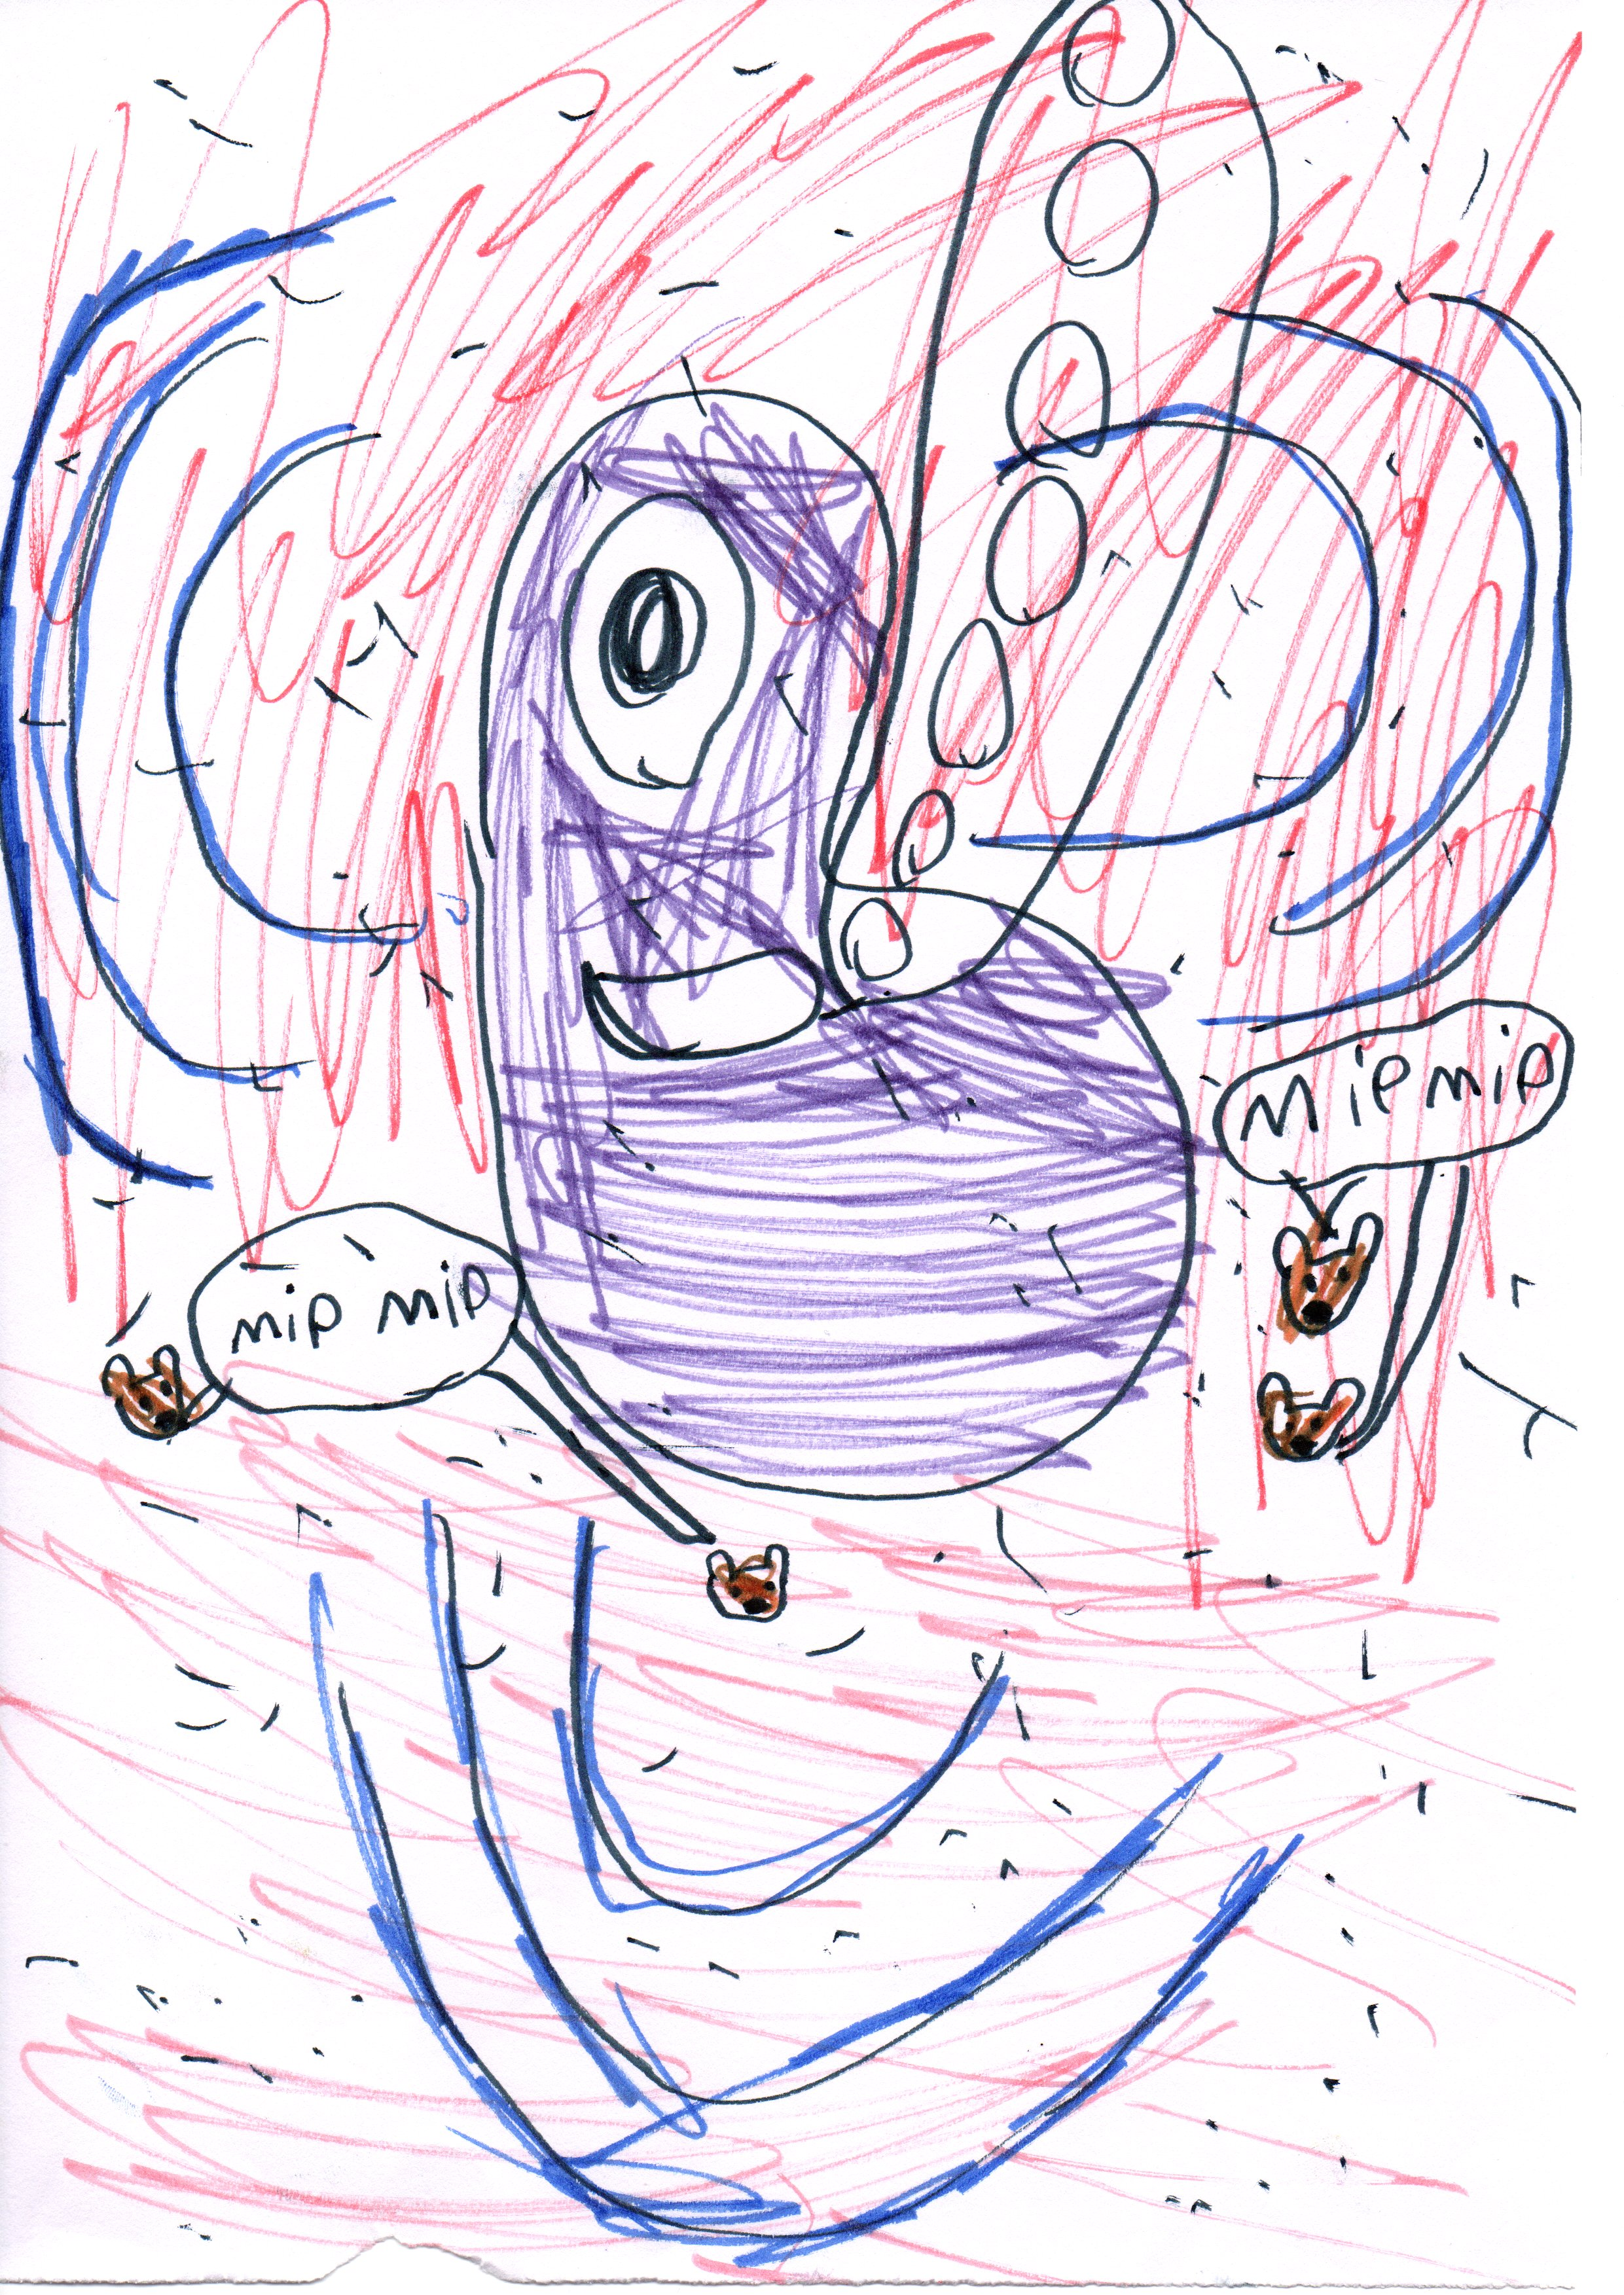
\includegraphics[scale=0.30]{illustrasjoner/kallemonster.jpg}
   \label{kallemonster}
   \caption{Kallemonster av Helene}
Og det var et monster som het Mo monsteret og kalte på Mol.\hfill \newline 

\hfill \newline
\end{figure}
\begin{figure}[H]
    \centering
    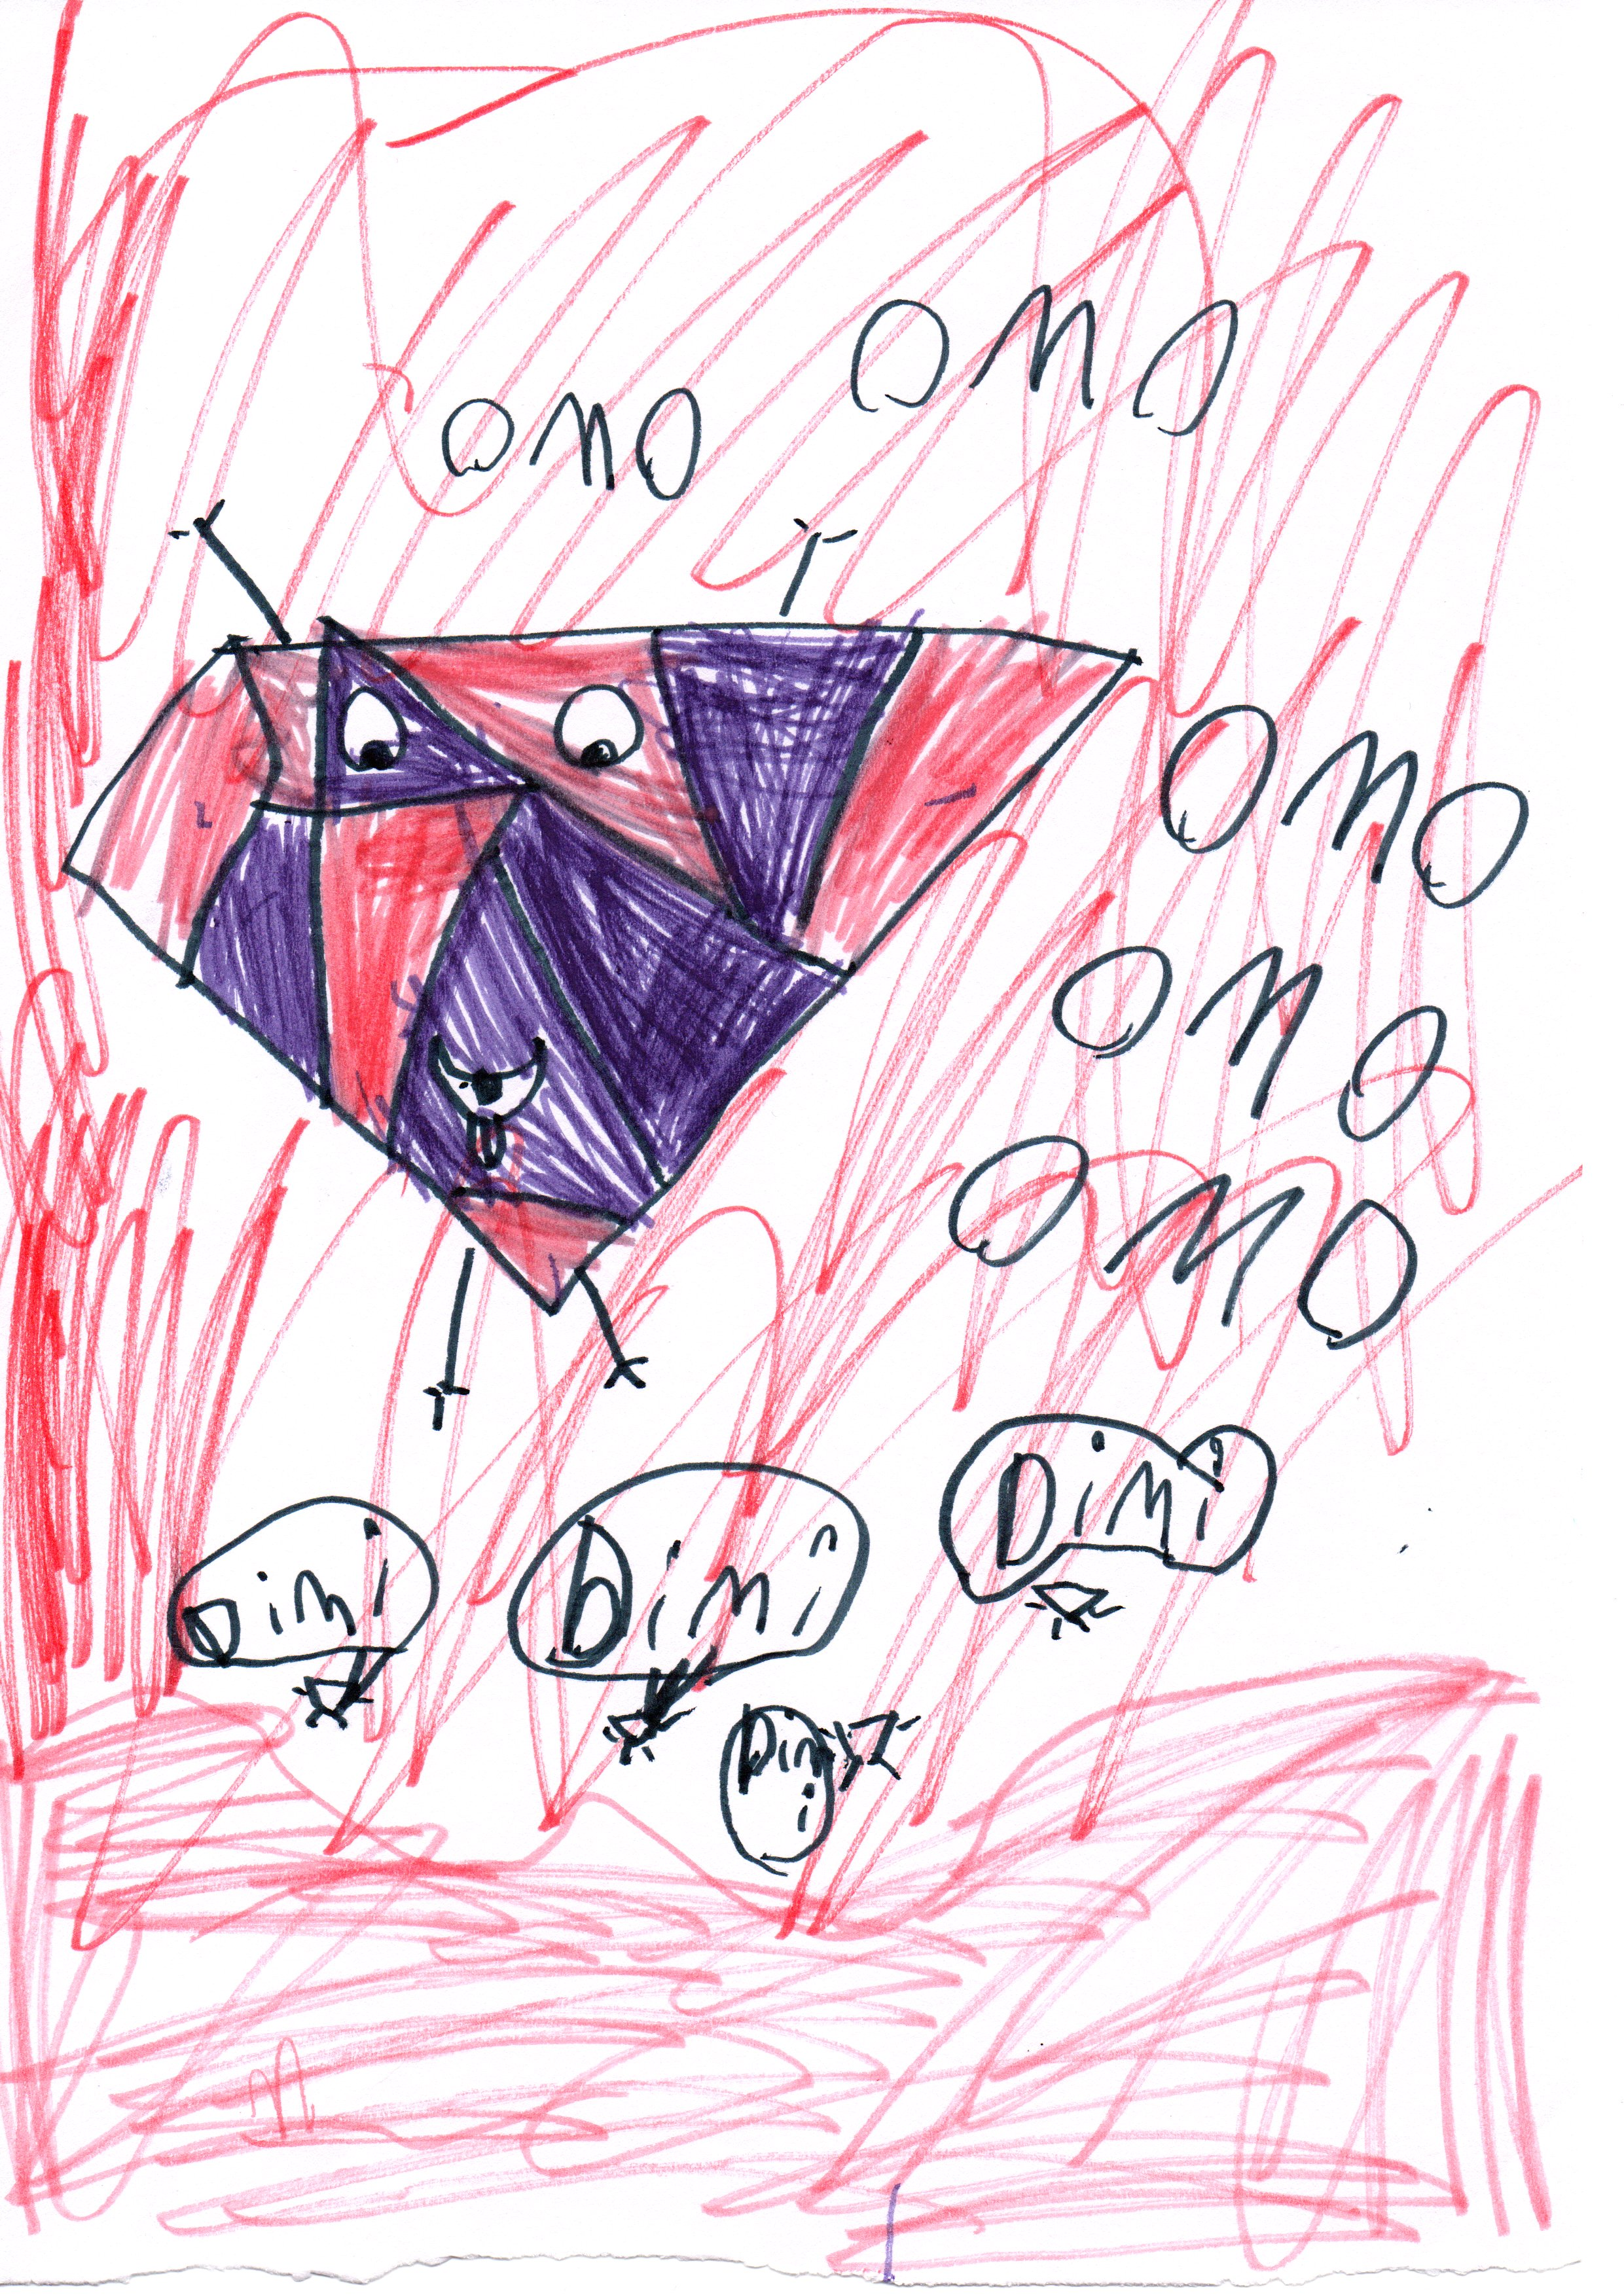
\includegraphics[scale=0.30]{illustrasjoner/omomonster.jpg}
   \label{Omomonster}
   \caption{Omomonster av Helene}
\end{figure}
Det var et monster som het Omo monsteret, og det var det største monsteret og kalte på Dimmi.\\
\hfill \newline 
\newpage
Hun reiste tilbake til Knask og godt, og der sto alle og ventet.\\ \hfill \\
Hun hadde med seg noen bamser og myke ting og litt glitter fra regnbue-planeten og hun fikk med seg noen diamanter til og lage andre og bedre matrealer fra monster-planeten og hun tok med seg noen fine ting fra Ferie-planeten.\\
\hfill \newline
Det kom plutselig et meteor-regn, men hun var alene så hun klarte ikke og stoppe det! \\
Men så kom monsterene og hjalp henne så de klarte og beskytte alle i byen!\\ \hfill \\
Hun var kjempe glad for at monsterene kom og hjalp til med meteorene som kom. Hun var så glad for at hun hadde oppdaget dem, virkelig kjempeglad!!
\begin{figure}[H]
    \centering
    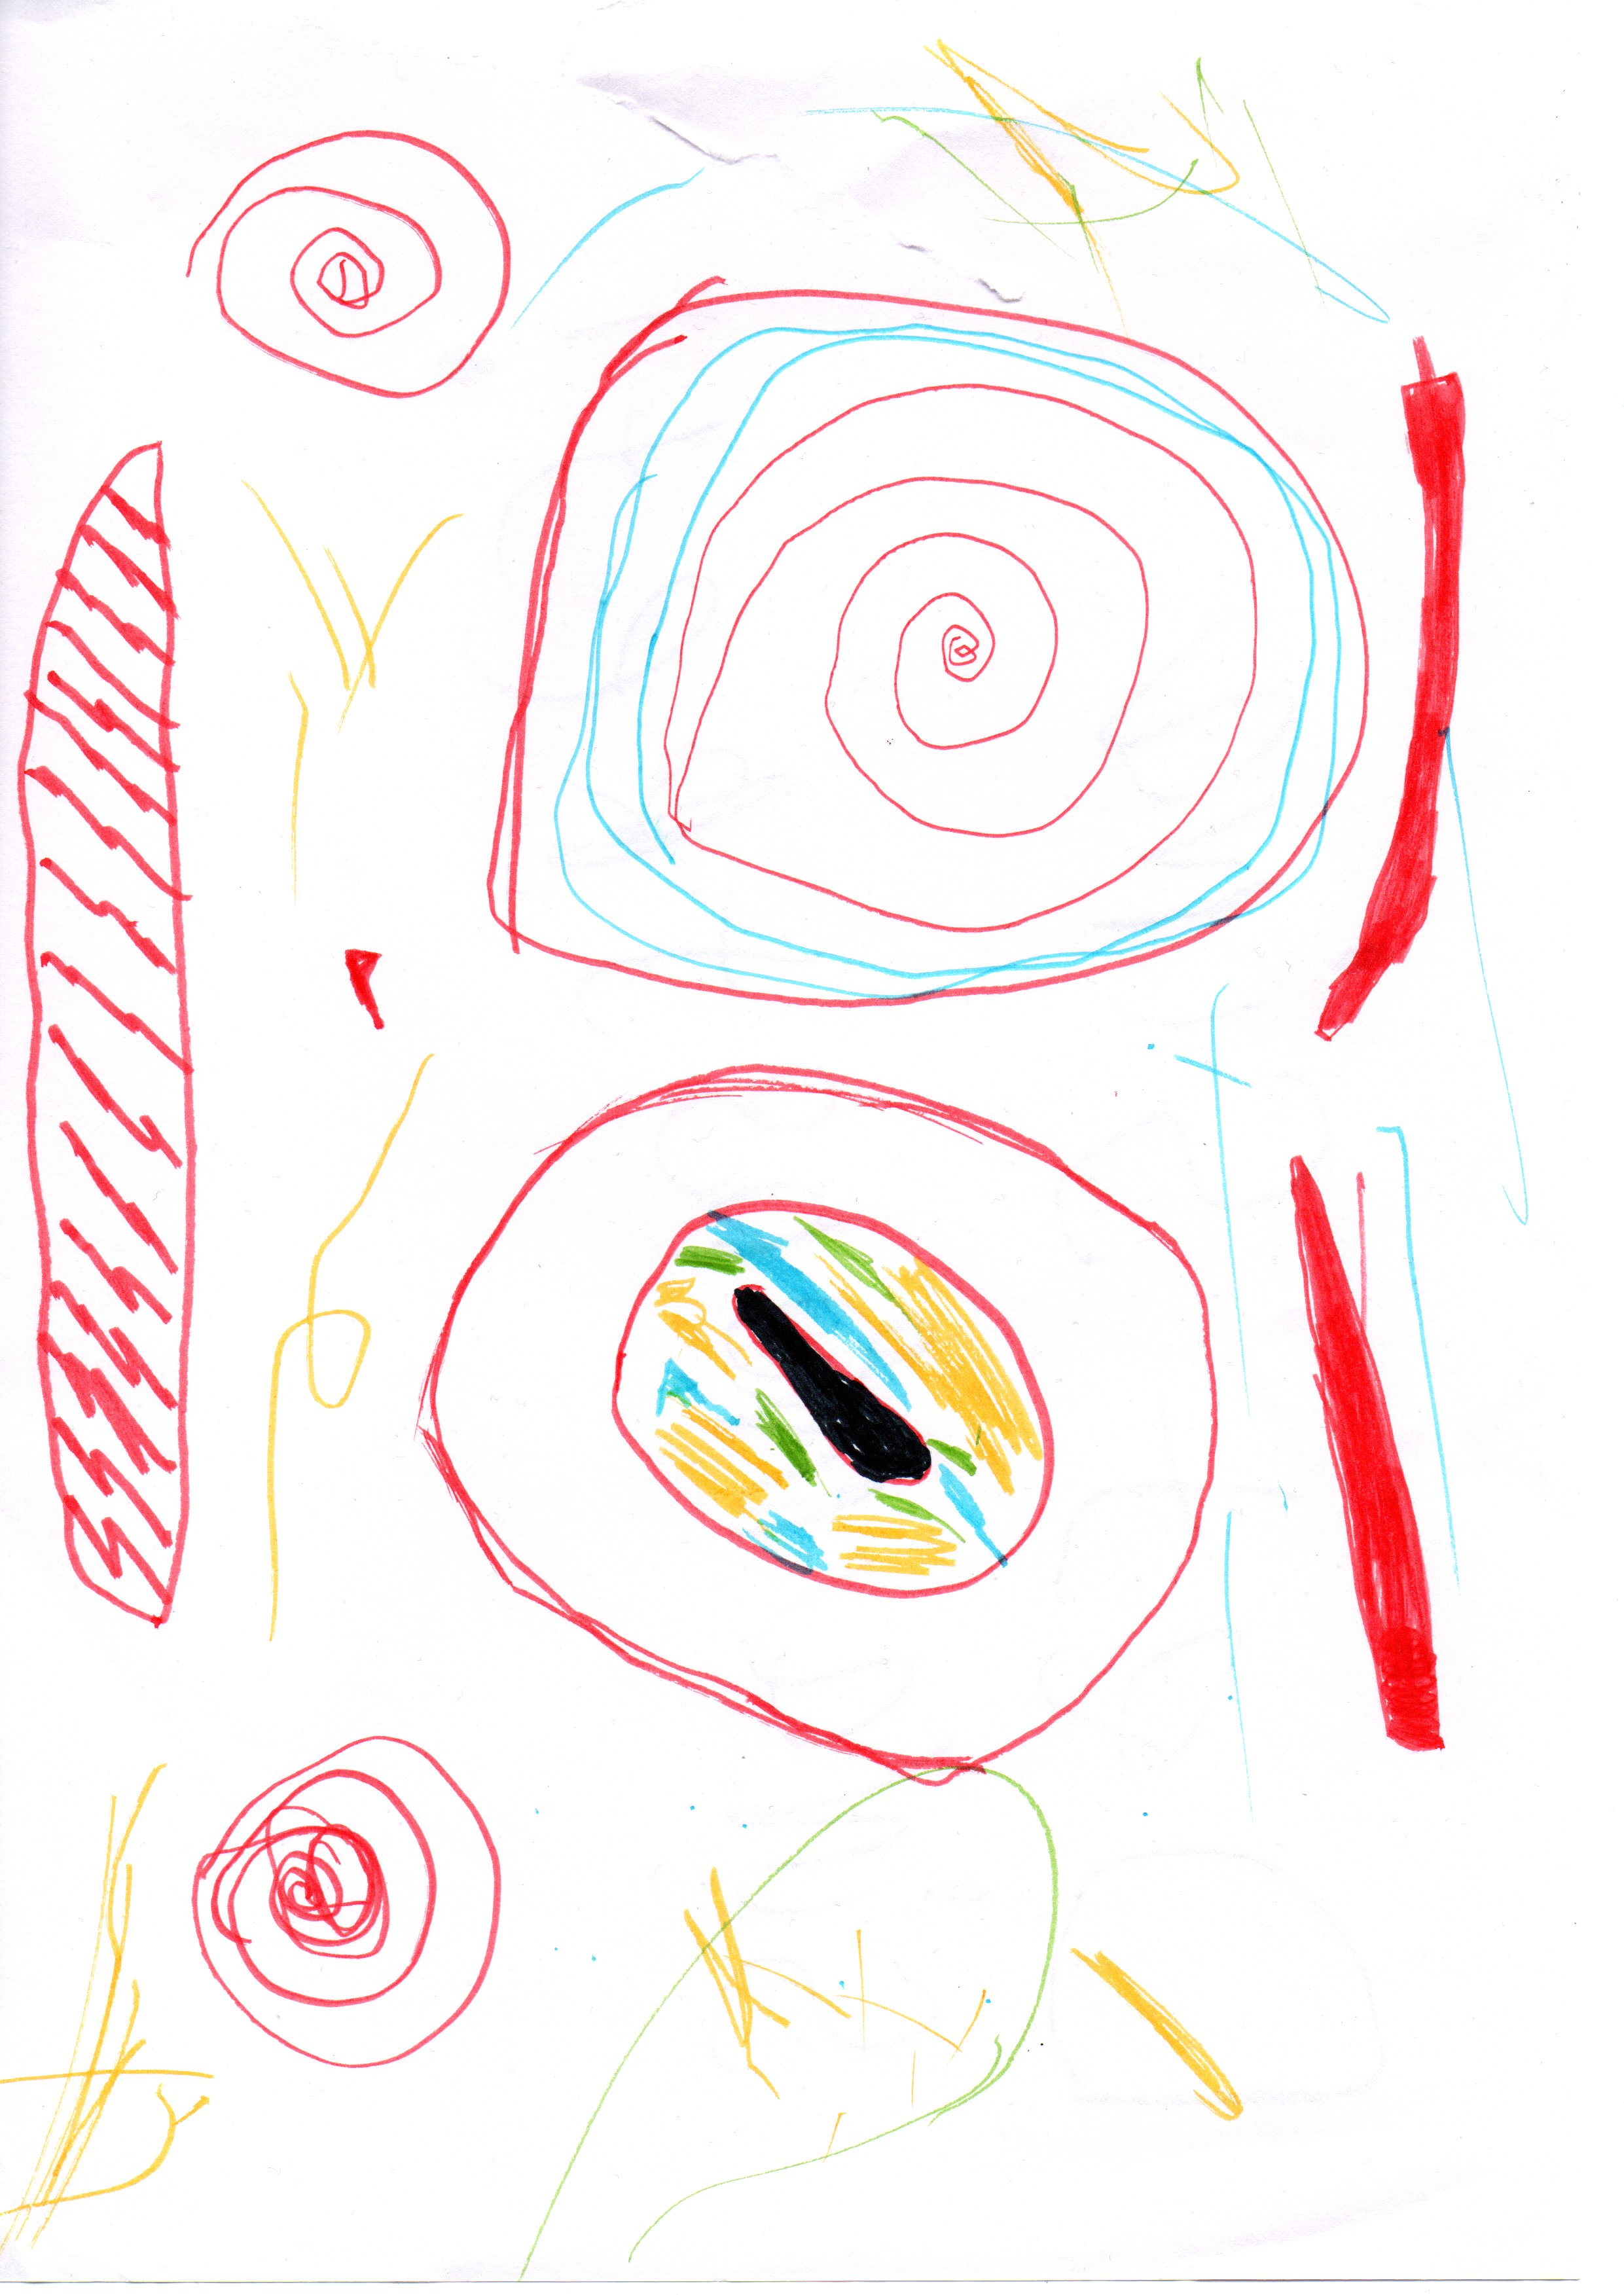
\includegraphics[scale=0.45]{illustrasjoner/Sinnasinnamonsteret.jpg}
   \label{Sinnasinnamonster}
   \caption{Sinnasinnamonster av Helene}
\end{figure}
\begin{figure}[H]
    \centering
    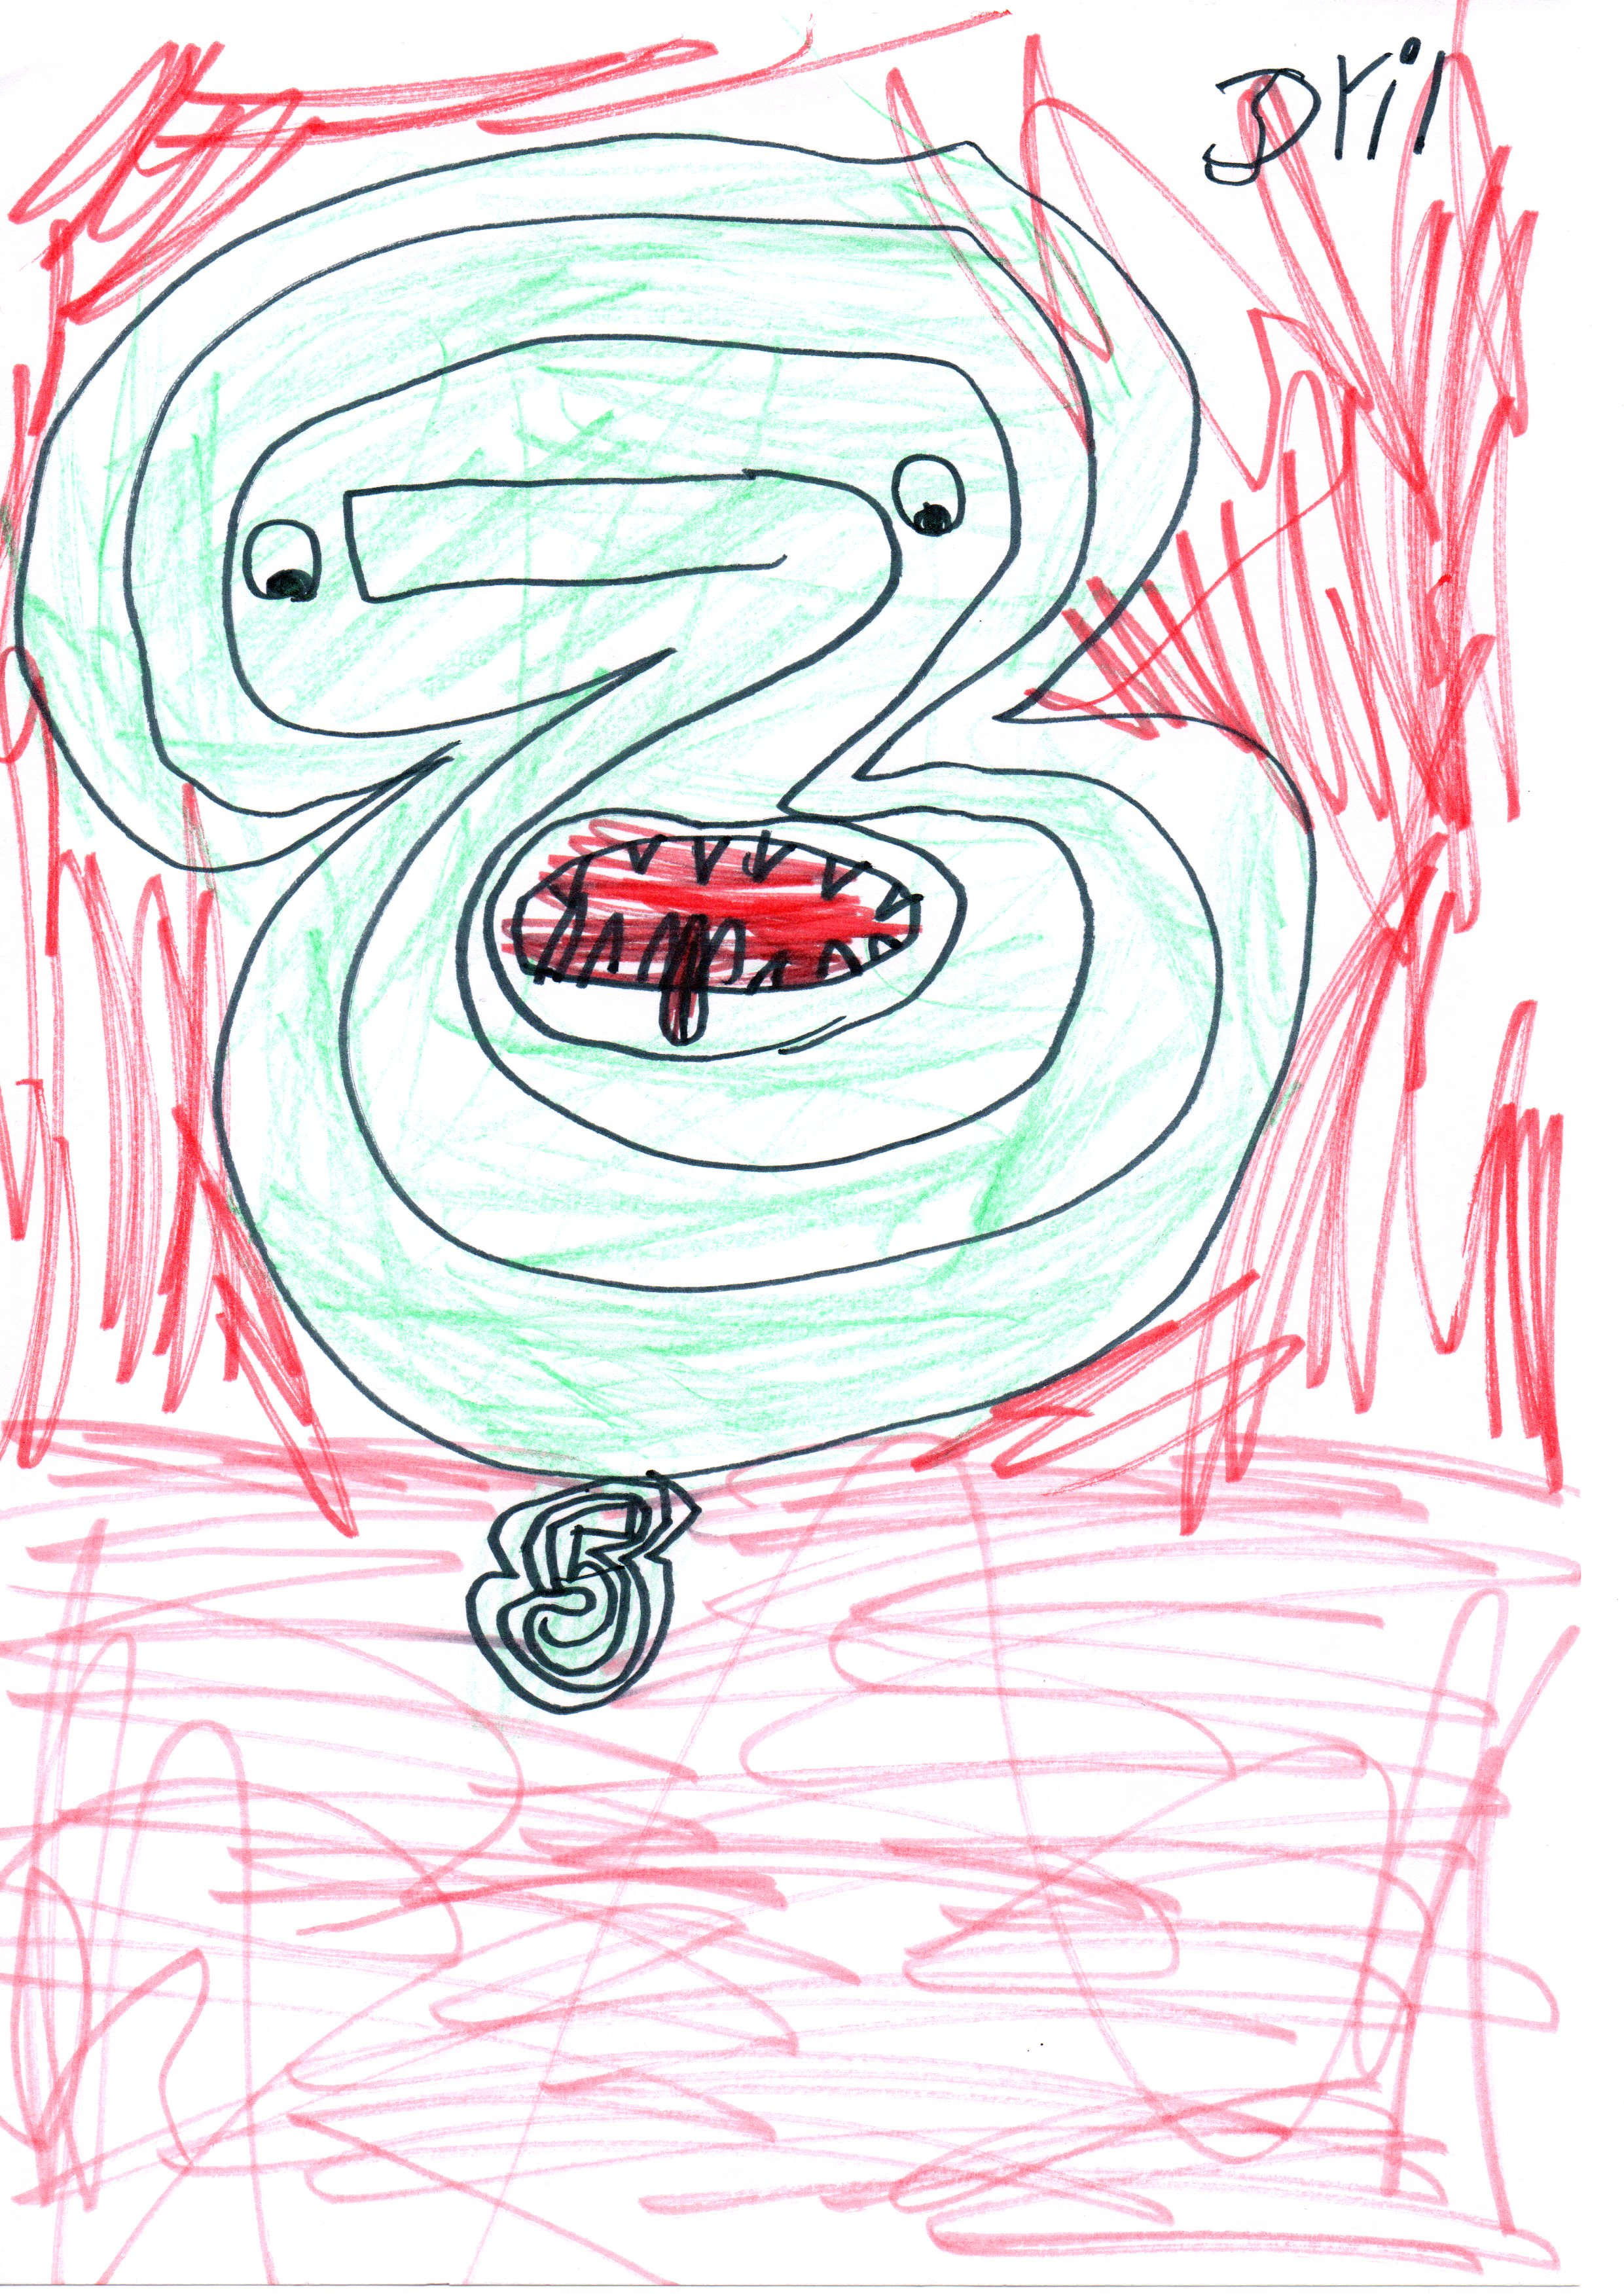
\includegraphics[scale=0.45]{illustrasjoner/groennslangemonster.jpg}
   \label{Grønnslangemonster}
   \caption{Grønnslangemonster av Helene}
\end{figure}
\section{Bortføringene på Knask og godt}
Hun dro til planeten jorden og fortalte alle hva som hadde skjedd men ingen trodde på henne så hun dro for og hente de levende seigmennene men det var ingen der men det var en liten barneseigmann som var der og latet som han var borgemesteren og hadde gullsmykke og han hadde stjelt pengene til alle i byen og sa: \textit{kom slaver}, men det kom ingen slaver. \\
Hun spurte han om hva som hadde skjedd han sa at det var en veldig fin melodi dem ble tiltrukket til og så spurte hun hvordan han ikke ble tiltrukket til melodien han svarte at han hadde headsett og hørte på en annen musikk. Da spurte hun om han viste hvem som hadde spilt musikken. Han viste ikke, men så at seigmennene hadde gått mot et meteorittskip som forsvant så fort som lysets hastighet. Hun spurte hvilken vei dem dro han svarte at skipet gikk til venstre og at hun måtte dra etter det sammen med han så han kunne vise vei. \\
\hfill \newline
Etter hvert så kom de til et sted med rød himmel istedet for et med svart, da skjønte dem at de nærmet seg. \\
Så så de et sted der seigmennene var slaver for aliens! Da skjønte de at dette kunne bli et farlig oppdrag. \\
Hun måtte finne på en god plan, så hun snek seg ned til aliensene.  Aliensene var så mange at mormor måtte få tak i hjelp. Hun dro til monster-planeten, men det var ingen monster der. \\
Det sto et skilt på planeten og der sto det at monsterene var på ferie på Ferie-planeten. Da dro hun til ferie-planeten, men planeten var så stor at det kom til og ta lang tid og finne monsterene. Hun letet og letet, men til 
slutt ga hun opp letingen. \\
Da måtte hun finne ut hva svakheten til aliensene var, så hun dro tilbake til der det var rødt og mørkt. \\
Hun stilte seg intil vinduet og der så hun at konge-alienen var ikke en alien, men en musketur. Musketuren lignet på en hund. Han eller hun latet som han var søt, men nor noen kom og klappet han så ble han et stort og skummelt monster med store hoggtenner og skarpe klør. \\
Hva skulle hun gjøre nå? Men så kom hun på at i det ødelagte romskipet var det gangsterbriller og militær klær og en pistol. Men hvordan skulle hun komme seg tilbake uten og ha blitt sett? Hun sukket lavt for seg. Hva skulle hun gjøre?\\
\hfill \newline
Hun lagde et stort hus. Hun ble der ganske lenge, men til slut hadde hun samlet inn nok info om musketurene. Hun klede seg ut som en alien. Ingen alien merket det. Så hun snek seg in til kongen og sa \textit{noen har stjålet bilen din}.  Plutselig fikk kongen hastverk med å kome seg bilen sin. Da måte mormor jåbe fort da hun hade kommet seg ned til fangehullet.
Og der var ale seigmennene, men vor var vakten som skal pase på fangene? \\
Men der var han! \textit{Han sover}, sa en av seigmennene \textit{og der er nøklene}.\\
Nøklene hang fast i belte hanes, men da tok mormor et sovemidel som hun spraiet onklig got. Hun lirket forsiktig nøkelen ut av beltet til vakten, og fikk ale seigmennene ut. Men hvordan skulle hun få alle tilbake uten å bli opdaget? Så kom på at hun hade røykbomber og røyksyn så hun kastet.



\chapter{Minner og hilsener}

%\begin{figure}[ht]
%    \centering
%    \includegraphics[width=1\textwidth]{Bryllupssang_fra_Erik.jpg}
%   \label{bryllupssang}
%    \caption{Brylllupssang skrevet av Gerds lillebror Erik}
%\end{figure}


\end{document}
